\section{Security Analysis}
\label{sec:securityAnalysis}

In this section, we perform an informal security analysis of \name. We split the security analysis in three separate parts. First, we show how isolation from a malicious OS and other malicious \sphw is achieved. Then we analyze the attacker-controlled life cycle events of \nameenclave{}s, and finally, we discuss the security of platform-wide attestation. 

\subsection{Isolation}

\subsubsection{Malicious OS}

In \name{}, the address regions that are used by \nameenclave{}s are protected using PMP entries~\cite{riscv2019privspec}. 
% This includes the private memory of processor-local enclaves and all shared memory regions. 
Recall that in stock keystone~\cite{keystone}, PMP is based on the physical memory range and only allows the specific enclave to access its private memory. On top of this, we use additional PMP entries to protect shared memory regions. 
% Hence, only the participating enclaves can access the shared memory regions. 
Note that only the highest privilege level, i.e., the SM, can modify PMP entries. During a context switch, the SM re-configures all PMP entries such that the correct memory ranges are available again. The SM has the complete overview over all enclaves and shared memory regions and sets up all PMP entries on its own. The processor will throw an access fault exception upon any memory access into protected memory regions. The hardware page table walker also must behave according to the configured PMP rules. Therefore, miss-configured page tables cannot be used to leak any data from protected memory ranges.

The SM enforces a shared memory region to be strictly shared between two entities (e.g., a processor-local enclave and a \sphw device). The SM also verifies that no overlap exists between the memory ranges similar to the stock keystone. 
%Thus, we only had to introduce minimal changes to add these new checks for shared memory. 

\subsubsection{Rogue DMA requests}
Malicious peripherals can try to access protected memory through rogue DMA requests. 
Mechanisms to restrict DMA requests already exist in other architectures, e.g., AMD IOMMU~\cite{amd2007iommu}, Intel VT-d~\cite{abramson2006vtd}, and ARM SMMU~\cite{arm2013smmu}. These mechanisms process every DMA request and verify its validity according to some access policy. Any memory access attempt that does not fit the access policy is blocked. Currently, the RISC-V standard does not contain a mechanism to limit such DMA requests. However, an input-output variant of a PMP called IOPMP~\cite{IOPMP} is an upcoming proposal in RISC-V. IOPMP enforces the configured PMP rules for non-RISC-V peripherals. Since our current prototype does not have any peripheral interface open to DMA requests, we do not need such protection. However, platforms that support DMA could implement mechanisms like IOPMP.

\subsubsection{Malicious application or controller enclaves}
The attacker-controlled OS can spawn malicious \app{}s and \ce{}s. Users remotely attest before providing any secret to the \app. During the platform-wide attestation, the user checks the attestation report of both the \app and \ce and aborts if they do not match with the intended enclave measurements. The platform-wide attestation also reveals any misconfiguration of communication links by an adversary. Note that this only verifies the static configuration of communication links. Upon any change to this setup, the external verifier might need to re-attest (c.f. \Cref{sec:security:lifecycleevents}). 

We require the \ce{} to provide isolation between multiple connected \app{}s (c.f. \ref{sec:programmingModel:systemComponents:multiApp}). Hence an attacker-controlled \app cannot access the confidential data of other \app{}s in the same \ce{}s.

Vulnerabilities within any of these enclaves could break the isolation guarantees of the data in that specific enclave. However, such an attack remains contained in the compromised enclave and cannot spread to connected enclaves. E.g., if a vulnerability in a \ce{} is found, only the data within that enclave is revealed. Any data that does not pass through the compromised \ce remains confidential. In this way, we provide defense-in-depth and reduce the potential impact of vulnerabilities.

\subsubsection{Malicious \sphw}
If an adversary manages to compromise the exact device that is used by an enclave, then any data on the \sphw is forfeit. However, any data not passed to the malicious device remains confidential.

We stress that certain manipulations of specific peripherals are always possible for an adversary. Consider, for example, a temperate sensor. Any local physical adversary can increase the real-world temperature and thus manipulate the sensor reading. However as we describe in our attacker model in Section~\ref{pie:sec:problemStatement:attackerModel}, the physical attacker is out-of-scope of this chapter. Note that this only applies to sensors, accelerators cannot get tampered with in this manner.

\subsubsection{Side channel attacks}
While we do not evaluate any defenses against side channel attacks, we discuss potential side channel attacks against our proposal and how they could potentially get mitigated. Many parts of \name{} remain the same as in traditional TEEs where side channels have been widely investigated~\cite{brasser2017software,brasser2019dr,gruss2017strongsidechannel}, however, we note that \name{} creates some new side channels that may not be present in traditional TEEs such as bus contention. 

\setcounter{para}{0}
\mypara{Traditional side channel attacks against TEEs}
Microarchitectural side channels in traditional TEEs leverage shared resources such as the cache~\cite{brasser2017software}, branch predictor~\cite{lee2017inferring}, and memory translation~\cite{xu2015controlled}. There exist several defenses against such attacks. Spatial partitioning of the cache in the form of cache coloring can fully defend against all cache based side channel attacks~\cite{costan2016sanctum,zhang2009cachecoloring,zhaosonicboom}. Similarly, other proposals have called for cache randomization~\cite{brasser2019dr,werner2019scattercache}. Processor features such as transactional memory have also been shown to mitigate cache attacks with low overhead~\cite{gruss2017strongsidechannel}. To the best of our knowledge, all of these proposals can be applied to \name{} due to the similar internal structure to traditional TEEs.

% Other RISC-V implementation such as SonicBOOM~\cite{zhaosonicboom} provides an out-of-order architecture that provides a number of side channel protections such as cache partitioning, cache timing obfuscation etc.\aritra{we can expand this by saying how the other RISC-V implementations can mitigate some of the side channel attacks.} 

\mypara{Side channel attacks within \sphw}
\Sphw contain shared resources such as caches, and thus are equally vulnerable as the processors~\cite{naghibijouybari2018rendered,ramesh2018fpga,visor}. However, mitigating these attacks is an orthogonal problem.

\mypara{Bus contention}
The introduction of peripherals into TEEs also implicates the bus as a new shared resource. An adversary could measure the throughput of her connection over the bus and observe any contention on the bus leading to less throughput.
Bus contention, however only exposes the access patterns of the peripherals. In extreme cases, the timing of bus contention could leak data, e.g., one side of the branch performs bus accesses while the other does not. However, in normal cases, the data between the peripherals and their corresponding processor-local enclaves usually remains inaccessible to the attacker.


% However, various techniques could be applied to \name{}s, such as cache partitioning~\cite{costan2016sanctum,zhang2009cachecoloring}. \name{} adds additional components, e.g., \ce{}s, that must be protected from any leakage. We believe that all additions of \name{} can be protected from side-channel attacks in a similar way as traditional TEEs~\cite{visor,brasser2019dr,costan2016sanctum}. However, more research is needed in this direction.

\subsection{Lifecycle events}
\label{sec:security:lifecycleevents}
As described in \Cref{sec:lifeycle}, there are two additional events for platform-wide enclaves in \name{}. \texttt{Connect} is used to connect two entities over a shared buffer. \texttt{Disconnect} facilitates a disconnect between the two enclaves. The \texttt{disconnect} is split into a synchronous and a asynchronous event. The asynchronous disconnect only occurs when one of the entities unexpectedly dies and results in the transfer of the sole ownership of the memory region to the remaining enclave. This enclave can then try to continue its execution. However, it will realize that the other entity has died as it does not react to any activity on the shared memory region. At a later point, the untrusted OS can issue a synchronous disconnect to notify the enclave and free the shared memory officially. Note that the SM mandates a synchronous disconnect before another \texttt{connect} command. Due to this architecture, a stale shared buffer will never be made accessible to any untrusted entity until a synchronous disconnect occurs, during which the enclave will officially get notified. The separate handling of synchronous and asynchronous disconnect events enforces protection for any secret data during an enclave's entire life cycle.

\subsection{Attestation} 

When the remote verifier attests to an enclave, he receives identifiers of all the connected enclaves. The SM generates these identifiers and makes sure that no two running enclaves share same identifier. Hence, an enclave could be assigned with an identifier that belonged to an enclave in the past. Of course, strictly increasing identifiers implemented with monotonic counters could be used for the identifier but such a solution needs a non-volatile storage on the CPU that is expensive. 

Now assume that the adversary kills an enclave and lunch another enclave with a \emph{different} binary (defined as \texttt{code}), but with the exact same identifier. . I.e., she can kill enclave $A$ and launch $A'$ (\texttt{code($A')\neq$code($A$)}) with the same identifier (\texttt{ID($A$)$=$ID($A'$)}). However, when a remote verifier attests $A'$, he sees that the measurements mismatch as \texttt{code($A')\neq$code($A$)} and rejects it.

Lets assume a more complex scenario with two pairs of enclaves: $A, B$ and $A', B'$, where $\textsf{code} (A')\neq \textsf{code} (A)$ but $\textsf{code} (B') = \textsf{code} (B)$. 
A remote verifier attests to an enclave $A$ that is connected to $B$ and and establishes a shared secret with $A$. Before the verifier attests to $B$, she kills $B$. The attacker then spawns a new enclave $B'$ where \texttt{ID($B$)$=$ID($B'$)}. The remote verifier will then attest to $B'$ and find that the code measurement looks fine. However, we stress that $B'$ cannot be connected to $A$ because then $A$ would need to receive a synchronous disconnect and would need to be re-attested (due to the configuration of $A$). Now the attacker kills $A$ and replace with $A'$ (where \texttt{ID($A$)$=$ID($A'$)}) and connect $A'$ and $B'$. The verifier then sees that $B'$ has the correct measurement and is connected to the identifier of $A$ (as \texttt{ID($A$)$=$ID($A'$)}). However, the verifier will want to provide its data to $A$ using the shared secret they have established in the previous attestation. Obviously, this cannot succeed as the new enclave $A'$ cannot know the secret.
 
% \begin{figure}
%     \centering
%     % 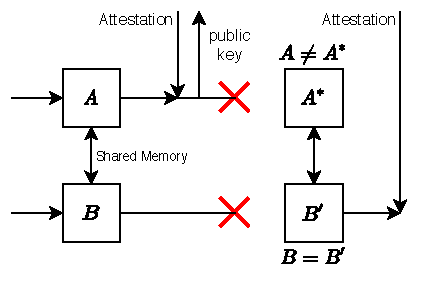
\includegraphics[width=0.7\linewidth]{images/sec-attestation.pdf}
%     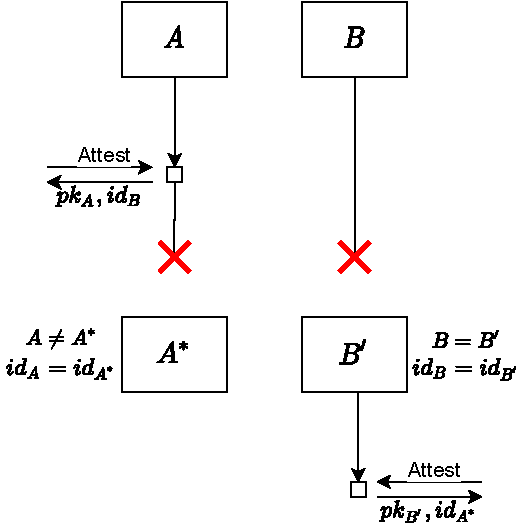
\includegraphics[width=0.7\linewidth]{images/sec-attestation-Page-2.pdf}
%     \caption{Caption\moritz{Does not really work}}
%     \label{fig:sec-attestation}
% \end{figure}
